\section{Method}

In this section, we propose the \textbf{P}otential-\textbf{R}esidual \textbf{I}ntegration for \textbf{M}ulti-threshold \textbf{E}ncoding (\textbf{PRIME}) framework, which optimizes the multi-threshold paradigm along two complementary dimensions: a more expressive encoding strategy and an inference-oriented hardware design tailored to it.

At the encoding level, PRIME introduces Integration Coding together with its companion Residual Membrane Potential Amplification (RMPA) mechanism, which progressively doubles the residual membrane potential so that MTNs deterministically recover previously unencoded information, achieving rapid convergence toward the corresponding ANN activation values.

At the inference level, PRIME co-designs spike generation and multiplication around the bit-level structure of FP16 operands: Direct FP16 Binary Parsing maps the sign, exponent, and mantissa fields directly to thresholds and spikes via a leading-one detector, while spike-driven multiplication reduces the mantissa product to trace-aligned shift-add operations, eliminating the usage of multipliers.

\subsection{Preliminary}
\label{sec:pre}

Following the successful practice of many prior works~\cite{you2024spikezip,wang2022signed,huang2025differential,huang2024towards}, in this paper, we adopt ternary-spike-based MTNs with outputs in $\{-1, 0, +1\}$ as the core computational unit of the SNN. Throughout this paper, we use the following notation: $t \in \{1, \ldots, T\}$ denotes the timestep index, where $T$ is the total number of timesteps; $i$ indexes the threshold within an MTN and also the amplification loop in RMPA; and $D$ denotes the intra-timestep spike dimension, i.e., the number of consecutive mantissa bits read per timestep.
Each MTN in layer $\ell$ is characterized by a base threshold $\theta^\ell$ and $2n$ thresholds, comprising $n$ positive and $n$ negative ones. The $i$-th threshold in layer $\ell$, denoted $\lambda_i^\ell$, is defined as $\lambda_i^\ell = \theta^\ell / 2^{i-1}$ for the positive branch ($i = 1, \ldots, n$) and $\lambda_{n+i}^\ell = -\theta^\ell / 2^{i-1}$ for the negative branch ($i = 1, \ldots, n$), forming a symmetric set of geometrically decaying values around zero.

Most ANN-to-SNN  methods are built upon rate coding~\cite{you2024spikezip,wang2022signed,wang2026training}. The neuronal dynamics of rate-coding-based MTNs can be described as the following equations: 
\begin{equation}
\begin{aligned}
\mathbf{m}^\ell[t] &= \mathbf{V}^\ell[t-1] + \mathbf{I}^{\ell}[t], &\quad
\mathbf{S}_i^\ell[t] &= \mathrm{MTH}_{\theta,n}(\mathbf{m}^\ell[t], i), \\
\mathbf{X}^\ell[t] &= \sum_i \mathbf{S}_i^\ell[t]\,\mathbf{W}^\ell \lambda_i^\ell, &\quad
\mathbf{V}^\ell[t] &= \mathbf{m}^\ell[t] - \mathbf{X}^\ell[t],
\end{aligned}
\end{equation}
\begin{equation}
\mathrm{MTH}_{\theta,n}(\mathbf{m}^\ell[t], i) = 
\begin{cases}
1, & \text{if } i = i^*(t) \text{ and } \mathbf{m}^\ell[t] \notin (\lambda_{2n}, \lambda_n), \\
0, & \text{otherwise},
\end{cases}
\end{equation}

where $\mathbf{m}^\ell[t]$, $\mathbf{V}^\ell[t]$, $\mathbf{I}^\ell[t]$, $\mathbf{S}_i^\ell[t]$, 
$\mathbf{W}^\ell$ and $\mathbf{X}^\ell[t]$ denote the pre-spike membrane potential, 
post-spike membrane potential, input current, output spike of the $i$-th 
threshold, weight, and total output signal of layer $\ell$ at timestep $t$, 
respectively. Here $i^*(t) \triangleq \arg\min_{p \in \{1,\ldots,2n\}} 
|\mathbf{m}^\ell[t] - \lambda_p|$ denotes the index of the threshold closest to the 
current membrane potential, so that the MTN fires a spike on the $i$-th 
channel only when $i$ matches this nearest threshold and $\mathbf{m}^\ell[t]$ lies 
outside the dead zone $(\lambda_{2n}, \lambda_n)$. Under rate coding, the 
quantization error between the ANN activation and the SNN output arises 
from the residual membrane potential that remains below the firing 
threshold. \added{That is, the membrane potential accumulates the input signal $\mathbf{I}^\ell$ in each timestep, and the residual membrane potential below the threshold cannot generate the corresponding spikes. The quantization error between the ANN activation $\mathbf{I}^\ell$ and the SNN neuron output is expressed as}
\begin{addedblock}
\begin{equation}
\varepsilon  = {\mathbf{I}^\ell} - \frac{1}{T}\sum\limits_{t = 1}^T {{\mathbf{X}^\ell}[t]}.
\end{equation}
\end{addedblock}
\added{The detailed error analysis is given in Section~\ref{sec:error-analysis}.}
Existing methods mitigate this error by increasing the number 
of timesteps or thresholds, both of which incur additional memory, 
computation, and energy overhead, thereby impeding edge deployment. To 
address this, we propose integration coding-based MTNs, which directly 
exploit the residual membrane potential without requiring extensive 
time-step iterations or a large number of thresholds.

\subsection{Multi-Threshold Neuron Based on Integration Coding}
\label{sec:method-ic}

\begin{figure}[htbp]
    \centering
    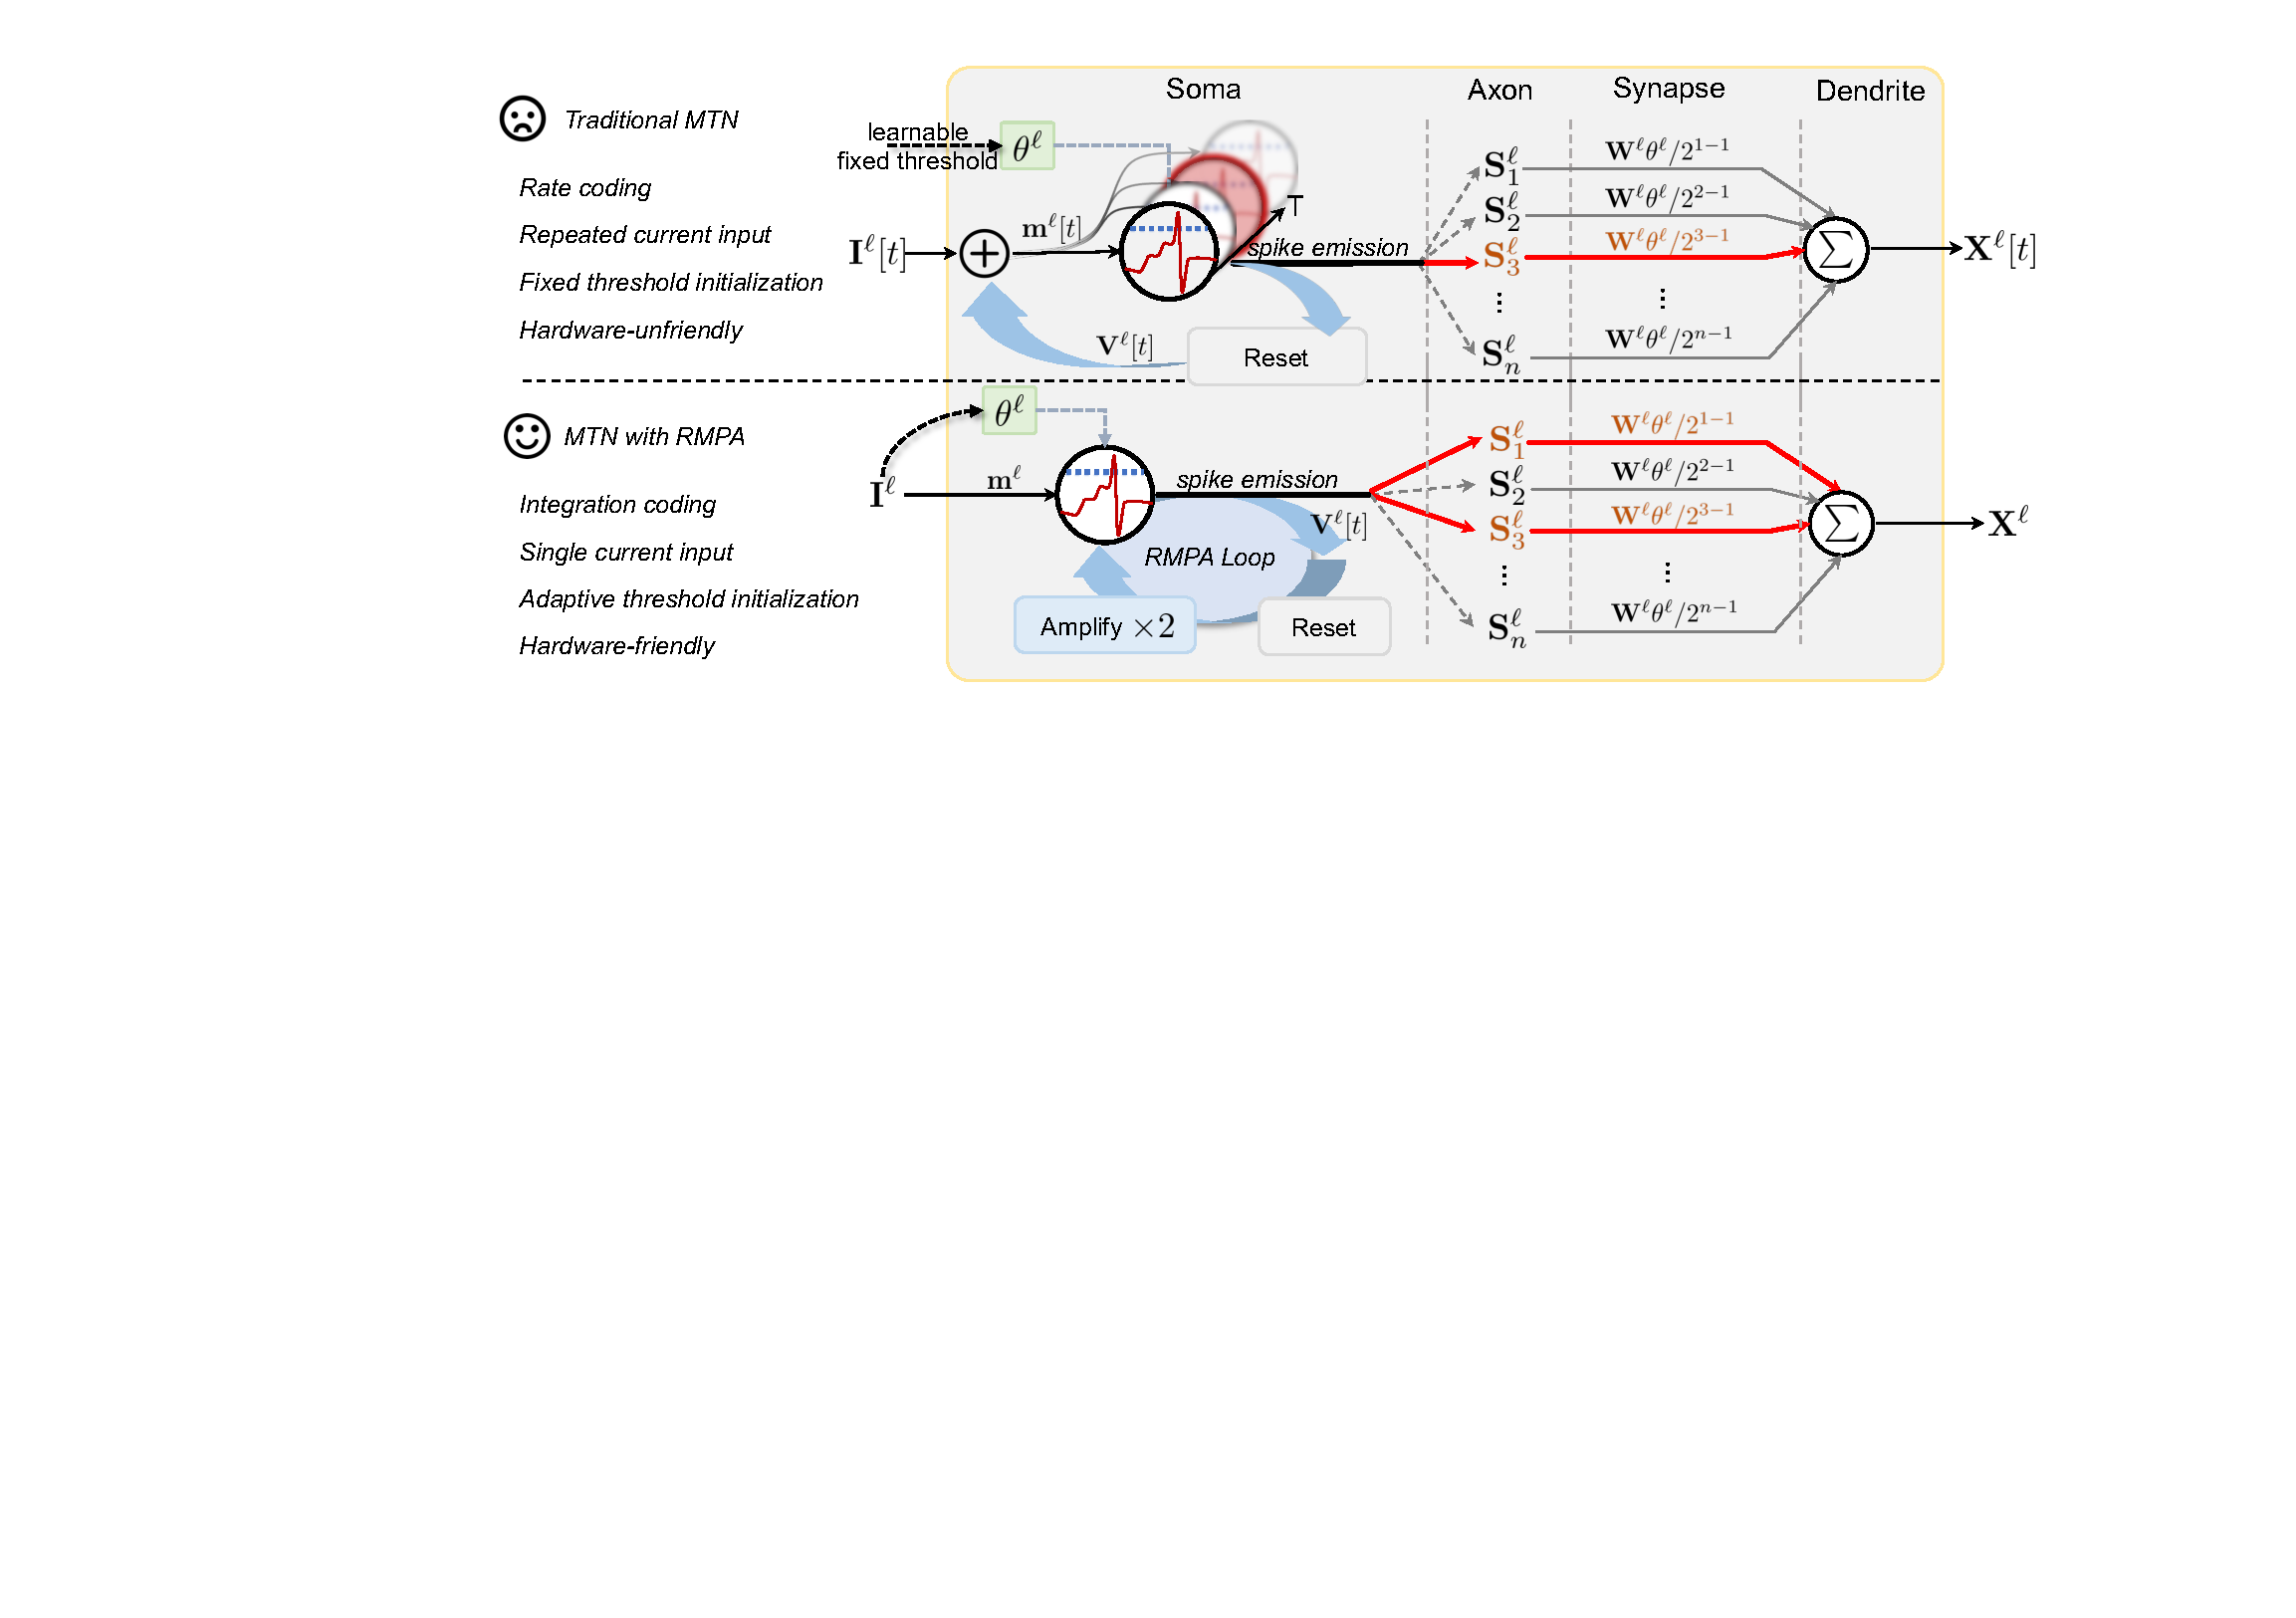
\includegraphics[width=1.0\linewidth]{Figs_new/01-neuron.pdf}
    \caption{Comparison between the traditional MTN and the proposed MTN with RMPA. \textbf{Upper}: For the traditional MTN, the input current is injected at each timestep, necessitating repeated accumulation operations of the input. 
    The neuron maintains $2n$ pre-set thresholds and compares its membrane potential against all of them to determine which spike to fire. 
    This results in redundant storage and computational overhead for threshold comparison per time step. 
    \textbf{Lower}: For the proposed MTN with RMPA, the input current is injected only once at the beginning, requiring no additional accumulation operation. 
    Instead of comparing against multiple thresholds, the neuron adaptively sets the only threshold $\theta^\ell = 2^p$ based on the input strength (Eq.~\ref{eqa:thres}). 
    At each timestep, a spike is fired if the residual potential after doubling exceeds $\theta^\ell$.
    Thus, only one threshold comparison is required, greatly reducing the computational overhead and the storage overhead from $\mathcal{O}(n)$ to $\mathcal{O}(1)$.
    }
    \label{Integral_Coding}
\end{figure}

The dynamics of the integration coding-based MTN are illustrated in Figure~\ref{Integral_Coding}. Conventional rate coding-based neurons accumulate input current at every timestep, whereas the integration coding-based MTN receives input only once, so the input current $\mathbf{I}^\ell$ directly initializes the membrane potential $m^\ell = \mathbf{I}^\ell$.
Afterwards, the neuron identifies the largest 
threshold that triggers spike emission, aligned with the binary structure of floating-point numbers 
(\added{the detailed description is in Appendix}~\ref{sec:hw_details}\deleted{ (the detailed description is in  Subsection}~\ref{subsec:spike-gen-via-fp16-binary-parsing}\deleted{)}). At the beginning, the base threshold $\theta^\ell$ is set and followed by a soft reset according to Eq.~\eqref{eqa:thres}:
\begin{equation}
\label{eqa:thres}
\theta^\ell = 2^p \text{ where } p = \max\{p \mid 2^p \leq \mathbf{m}^\ell,\ p \in \mathbb{Z}\},
\end{equation}
\begin{equation}
\label{eqa:reset}
\added{\quad\mathbf{m}_{rest}^\ell =\mathbf{m}^\ell - \mathbf{S}_i^\ell \theta^\ell}
\end{equation}
\begin{equation}
\added{\quad\mathbf{V}^\ell =2\mathbf{m}_{rest}^\ell=\mathbf{m}_{rest}^\ell+\mathbf{m}_{rest}^\ell,}
\end{equation}
\added{Depending on the hardware form, this doubling can be implemented either by adding the membrane potential to itself or by multiplying it by 2.}
\begin{equation}
\deleted{\quad\mathbf{V}^\ell = \mathbf{m}^\ell - \frac{\mathbf{S}_i^\ell \theta^\ell}{2^{i-1}},}
\end{equation}
where $i$ indicates the loop index of RMPA.
In each subsequent iteration, $\mathbf{m}^\ell$ is set to the post-reset membrane potential $\mathbf{V}^\ell$.

The RMPA-based MTN iteratively generates sub-threshold spikes from the residual membrane potential, progressively reducing the quantization error. Each spike generation requires only a bit-shift and a single comparison against the base threshold $\theta ^\ell$, eliminating storing a large number of thresholds. Formally, the firing rule is defined as Eq.~\eqref{eqa:reset}:
\begin{equation}
\deleted{
\label{eqa:spike}
\mathbf{S}_i^\ell = \mathrm{MTH}_{\theta,n}(\mathbf{m}^\ell, i) = 
\begin{cases}
1, & \text{if } \mathbf{m}^\ell \cdot 2^{i - 1} - {\theta ^\ell} \ge 0\, \\
0, & \text{otherwise}
\end{cases}.}
\end{equation}
\begin{equation}
\added{
\label{eqa:spike}
\mathbf{S}_i^\ell = \mathrm{MTH}_{\theta,n}(\mathbf{m_{i-1}}^\ell, i) = 
\begin{cases}
1, & \text{if } \mathbf{m_{i-1}}^\ell - {\theta ^\ell} \ge 0\, \\
0, & \text{otherwise}
\end{cases}.}
\end{equation}
\added{That is, the residual membrane potential is doubled at each amplification loop, and a spike is fired when the amplified membrane potential reaches the base threshold $\theta^\ell$; the actual amplitude of the emitted spike is $\theta^\ell / 2^{i-1}$.}

\added{To enable efficient implementation on mainstream binary hardware, we additionally introduce the concept of $D$. $D$ denotes the intra-timestep spike dimension, i.e., the number of consecutive mantissa bits read per timestep, and the above firing rule corresponds to the basic case of $D = 1$. When $D > 1$, the encoding can also be realized in the form of spike emission: the residual membrane potential is amplified by $2^{D}$ at once,}
\begin{equation}
\added{\quad\mathbf{V}^\ell = 2^D \cdot \mathbf{m}_{rest}^\ell,}
\end{equation}
\added{and the emitted spike is the $D$-bit unsigned integer}
\begin{equation}
\added{\quad S = {\max\{s \in \{0, 1, \ldots, 2^D - 1\} \mid \mathbf{V}^\ell \ge s\,\theta\}}_2,}
\end{equation}
\added{representing 0 to $2^D - 1$ times the corresponding threshold. Between two timesteps, the membrane potential is further amplified by $2^{n}$ until $\mathbf{V}^\ell > \theta$, which describes the transition between successive timesteps. The setting of $D > 1$ is mainly designed to adapt to the current mainstream binary hardware forms, while it can also be applied on future neuromorphic chips.}

A soft reset is then applied as defined in Eq.~\eqref{eqa:reset}. Once the membrane potential reaches zero or the prescribed number of iterations is exhausted, the neuron decodes the emitted spike sequence to produce the total output signal of layer $\ell$:
\begin{equation}
{\mathbf{X}}^{\ell} = \sum_{i}\mathbf{S}_i^\ell \mathbf{W}^\ell \frac{ \theta^\ell}{2^{i-1}}.
\end{equation}
\added{Since $\theta^\ell = 2^p$ and $p$ is an integer, the weight-spike product satisfies $\mathbf{W}^\ell \cdot 2^{p-(i-1)}$, which can be implemented via bit-shifting, eliminating the need for explicit multiplication.}

\added{To further illustrate the dynamics of RMPA, a concrete example is provided here.} \movednote{(The example is moved from Appendix~\ref{sec:rmpa_example} of the previous version to the main text.)}
\moved{Consider an input $\mathbf{I}^\ell = 1.4$. According to Eq.~\eqref{eqa:thres}, the threshold $\theta^\ell$ is set to $1$ ($2^{p}$, $p=0$). After a spike of $\theta^\ell=1$ is emitted, it leaves $\mathbf{m}^\ell=1.4-1$ as $0.4$ and the index $i$ of RMPA loop as $1$. In the second iteration, $\mathbf{m}^\ell$ is doubled to $0.8$ and $i$ advances to $2$; since $\mathbf{m}^\ell = 0.8 < \theta^\ell=1$, no spike is emitted. In the third iteration, $\mathbf{m}^\ell$ is doubled to $1.6$ and $i$ advances to $3$; since $\mathbf{m}^\ell = 1.6 > \theta^\ell=1$, a spike of $\theta^\ell / 2^{i-1}= 0.25$ is fired and $\mathbf{m}^\ell$ is reset to $1.6 - 1 = 0.6$. At this point, the total encoded value is $1 + 0.25 = 1.25$, with residual membrane potential $\mathbf{m}^\ell = 0.6$. The remaining encoding error is $1.4 - 1.25$, the same as the result of $\mathbf{m}^\ell / 2^{i-1} = 0.6 / 4$, which decays exponentially with increasing iterations.}

Our proposed neurons offer two key advantages: (i) threshold storage is reduced from $2n$ to $1$, with a corresponding reduction in I/O operations; (ii) unlike rate coding, integration coding-based MTNs actively exploit the residual membrane potential to suppress quantization error, which is the fundamental source of the accuracy gain.

\deleted{To further illustrate the dynamics of RMPA, a concrete example is provided in Appendix~\ref{sec:rmpa_example}.}


\subsection{\added{Error Analysis}}
\label{sec:error-analysis}
\movednote{This subsection is moved from Appendix~\ref{sec:error} of the previous version to the main text, and the derivations are explained in detail.}

\moved{The conversion error in ANN-to-SNN algorithms arises primarily from residual membrane potential below the threshold that fails to generate corresponding spikes.}

\added{The error bounds of rate coding and the proposed encoding are summarized in the following proposition.}
\movednote{This proposition and the following paragraph are moved from the end of Subsection~\ref{sec:method-ic} of the previous version to here, merging the error analysis into this subsection.}
\begin{proposition}[\moved{Error Bound of RMPA-based MTN}]
\label{prop:rmpa-mtn-error-bound}
    \moved{The encoding error of rate coding is bounded by
    $\varepsilon_{\text{rate}} < \theta/2T,$
which decays linearly with $T$. In contrast, the proposed PRIME encoding attains a bound $\varepsilon_{\text{PRIME}} < \theta/2^{T \cdot D + 1}$, which decays exponentially with $T$, where $\theta$ denotes the spike threshold, $T$ the number of inter-timesteps, and $D$ the number of concurrent intra-timestep spikes.}
\end{proposition}

\moved{\deleted{The full proof is given in Appendix~\ref{sec:error}.} \added{The detailed derivation is given below.} Accordingly, the error bound of our proposed MTN is significantly tighter than that of conventional MTN: for instance with $T=2$ and $D=3$, the error bound of PRIME is $\theta / 2^{7} = \theta / 128$, which is $32\times$ tighter than the rate coding bound of $\theta / 4$.}
\added{Even when $D = 1$, the error bound is $\theta / 2^{T+1}$, which still decays exponentially with $T$.}

\movedparagraph{Conventional Rate Coding}

\moved{In conventional ANN-to-SNN conversion, the neuron accumulates the input signal $\mathbf{I}$ at each timestep:}
\begin{movedblock}
\[
\mathbf{m} \leftarrow \mathbf{m} + \mathbf{I}.
\]
\end{movedblock}
\moved{The membrane potential is then compared against the threshold $\theta$. If $\mathbf{m} > \theta$, a spike is emitted and the membrane potential is updated as:}
\begin{movedblock}
\[
\mathbf{m} \leftarrow \mathbf{m} - \theta.
\]
\end{movedblock}
\moved{After $T$ accumulation steps:}
\begin{movedblock}
\[
T \cdot \mathbf{I} = \theta \cdot N_{\text{spike}} + \mathbf{m}_{\text{rest}},
\]
\end{movedblock}
\moved{where $N_{\text{spike}}$ denotes the total number of emitted spikes. The ideal encoded value is $\mathbf{I}$, whereas the actual decoded value is:}
\begin{movedblock}
\[
\frac{\theta \cdot N_{\text{spike}}}{T} = \mathbf{I} - \frac{\mathbf{m}_{\text{rest}}}{T}.
\]
\end{movedblock}
\moved{The encoding error over $T$ steps is therefore:}
\begin{movedblock}
\[
\varepsilon = \frac{\mathbf{m}_{\text{rest}}}{T}, \quad \mathbf{m}_{\text{rest}} < \theta \implies \varepsilon < \frac{\theta}{T}.
\]
\end{movedblock}
\moved{With optimized initial membrane potential initialization, $\mathbf{m}_{\text{rest}} < \theta/2$ can be guaranteed~\cite{hao2023bridging}, yielding a tighter bound:}
\begin{movedblock}
\[
\varepsilon < \frac{\theta}{2T}.
\]
\end{movedblock}

\added{In other words, the decoded value differs from the ideal value only by the residual membrane potential divided by $T$. The residual membrane potential $\mathbf{m}_{\text{rest}}$ is smaller than $\theta$, and with optimized initial membrane potential initialization it is effectively less than $\theta/2$~\cite{hao2023bridging}; the error thus distributes within $\theta/2T$, which decays linearly with $T$.}

\movedparagraph{Proposed Integration Coding}

\moved{The method proposed in this paper adopts integration coding, where the input signal $\mathbf{I}$ is applied only at the first timestep:}
\begin{movedblock}
\[
\mathbf{m} = \mathbf{I}.
\]
\end{movedblock}
\moved{In subsequent steps, the residual membrane potential is amplified without further input injection. Let $n_i$ denote the amplification index at which the $i$-th spike is emitted; the corresponding spike amplitude is $\theta / 2^{i-1}$. After $n$ amplification operations, the input is decomposed as:}
\begin{equation}
%\begin{movedblock}
%\[
\added{
\mathbf{I} = \sum_{i_{where\, S_i =1}} \frac{\theta}{2^{i-1}} + \frac{\mathbf{m}_{\text{rest}}}{2^{n}},
}
%\]
%\end{movedblock}
\end{equation}
\moved{where the second term represents the residual encoding error. The encoding error is thus:}
\begin{movedblock}
\[
\varepsilon = \frac{\mathbf{m}_{\text{rest}}}{2^{n}}, \quad \mathbf{m}_{\text{rest}} < \theta \implies \varepsilon < \frac{\theta}{2^{n}}.
\]
\end{movedblock}
\moved{When the carry mechanism is applied, the error is further reduced by half:}
\begin{movedblock}
\[
\varepsilon < \frac{\theta}{2^{n+1}}.
\]
\end{movedblock}
\moved{Here, $n$ denotes the total number of amplification operations. When $T = 1$, we have $n = D$. When $T > 1$, additional amplification operations are required between timesteps to satisfy the condition $\mathbf{m}_{\text{rest}} > \theta$ prior to spike emission, yielding:}
\begin{movedblock}
\[
n \geq T \cdot D,
\]
\end{movedblock}
\moved{and the error is bounded by:}
\begin{movedblock}
\[
\varepsilon < \frac{\theta}{2^{T \cdot D + 1}}.
\]
\end{movedblock}

\added{That is, the first term $\sum_{i_{where\, S_i =1}} \frac{\theta}{2^{i-1}}$ is the value encoded by the emitted spikes, and the second term $\mathbf{m}_{\text{rest}}/2^{n}$ is the residual encoding error, which decays exponentially with the number of amplifications $n$. Compared with the error $< \theta/2T$ of rate coding, the error of the proposed method distributes within $\theta/2^{T \cdot D + 1}$, and thus the error distribution of the proposed encoding is significantly reduced.}

\subsection{Hardware-efficient Inference}
\label{sec:hw}
\movednote{This subsection is greatly simplified compared with the previous version; the detailed implementation, figures, and derivations are moved to Appendix~\ref{sec:hw_details}.}

Here we describe how the spike generation process is  bound to the binary representation of FP16 data, eliminating conventional membrane potential computation. The key is that each field of the FP16 format: sign, exponent, and mantissa can be mapped to the threshold and the spike corresponding to Eq.~\eqref{eqa:thres} and ~\eqref{eqa:spike}, enabling a purely read-based spike emission mechanism.

A normalized FP16 floating-point number is represented as:
\begin{equation}
    x_{\textbf{10}} = (-1)^{S} \times 2^{E-15} \times \left(1 + \sum_{j=1}^{10} M_j \times 2^{-j}\right),
\end{equation}
where $S$ is the 1-bit sign, $E$ is the 5-bit exponent ($1 \leq E \leq 30$), and $M_1 M_2 \cdots M_{10}$ is the 10-bit mantissa with an implicit leading 1. 
In the first cycle, the implicit leading 1 of the FP16 representation is directly emitted as the first spike, and the sign bit $S$ together with the exponent $E$ determines the corresponding threshold $\theta_1 = (-1)^{S} \times 2^{E-15}$. Starting from the second cycle, the position of the first 1 in the remaining mantissa is located using a leading-one detector (LOD), a well-established combinatorial logic module in digital circuit design. Unlike the traditional ANN-to-SNN approaches that require the full subtract-compare-conditional updates, this method simplifies each cycle to LOD lookups followed by a bit-clear operation, significantly reducing computational cost. \movednote{(The detailed description of spike generation, including the threshold $\theta_k = (-1)^{S} \times 2^{E-15-k}$, multi-bit spike emission with $D > 1$, the carry operation and the parallelism of $T \leq 2$, is moved to Appendix~\ref{subsec:spike-gen-via-fp16-binary-parsing}.)}

The spike generation mechanism described above decomposes an FP16 value into a sequence of weighted spikes over $T$ inter-timesteps. We now show how this decomposition naturally induces a hardware-efficient multiplication scheme: instead of performing a full $11 \times 11$-bit mantissa multiplication, the product $x \times w$ is computed incrementally through spike-driven conditional shift-add operations across timesteps. \movednote{(The detailed description of the sign and exponent processing, the mantissa decomposition, and the trace-aligned temporal accumulation is moved to Appendix~\ref{sec:hw_details}, and the multiplication example with $T=2$ and $D=3$ is shown in Figure~\ref{fig:calc}.)} \deleted{This temporal accumulation directly mirrors the dynamics of synaptic integration in SNNs: each incoming spike $s_t$ triggers a weighted response $F_{o}|_t$, and the trace $\mathrm{Tr}_t$ governs the temporal decay (realized here as a right shift) before the responses are accumulated at the output neuron.}

A key advantage of this binary-parsing approach is that when $T \leq 2$, the two timesteps are data-independent: the first reads the implicit 1 and leading mantissa bits, while the second operates on the remaining bits through a LOD. Since the second timestep depends only on a predetermined bit range, both can be executed in parallel, effectively halving the latency.

The Spike Generation via Direct FP Binary Parsing, together with the Spike-driven Multiplication, yields significant energy and data-transmission savings. The detailed energy analysis is given in Appendix~\ref{sec:energy}.
